\documentclass{article}
\usepackage{arxiv}
\usepackage{amsmath}
\usepackage[utf8]{inputenc}
\usepackage[english, russian]{babel}
\usepackage[T1]{fontenc}
\usepackage{url}
\usepackage{booktabs}
\usepackage{amsfonts}
\usepackage{nicefrac}
\usepackage{microtype}
\usepackage{lipsum}
\usepackage{amssymb}
\usepackage{graphicx}
\usepackage{natbib}
\usepackage{doi}

\pagestyle{fancy}



\title{Восстановление прогноза, сделанного в метрическом вероятностном пространстве, в исходное пространство (временных рядов)}

\author{ Maxim Divilkovskiy \\
% \thanks{Use footnote for providing further
% 		information about author (webpage, alternative
% 		address)---\emph{not} for acknowledging funding agencies.} \\
	Chair of Data Analysis\\
	MIPT\\
	\texttt{divilkovskii.mm@phystech.edu} \\
	%% examples of more authors
	\And
	Vadim Strijov \\
	FRC CSC of the RAS\\
	Moscow, Russia\\
    \texttt{strijov@phystech.edu} \\
    \And
    Yakovlev Konstantin \\
    Chair of Intellectual Systems\\
    MIPT\\
    \texttt{iakovlev.kd@phystech.edu} \\
	% Santa Narimana, Levand \\
	% \texttt{stariate@ee.mount-sheikh.edu} \\
	%% \AND
	%% Coauthor \\
	%% Affiliation \\
	%% Address \\
	%% \texttt{email} \\
	%% \And
	%% Coauthor \\
	%% Affiliation \\
	%% Address \\
	%% \texttt{email} \\
	%% \And
	%% Coauthor \\
	%% Affiliation \\
	%% Address \\
	%% \texttt{email} \\
}
\date{}

\renewcommand{\shorttitle}{\textit{arXiv} Template}

%%% Add PDF metadata to help others organize their library
%%% Once the PDF is generated, you can check the metadata with
%%% $ pdfinfo template.pdf
\hypersetup{
pdfauthor={Maxim Divilkovskiy},
}

\graphicspath{ {./figures/} }

\begin{document}
\maketitle

\begin{abstract}
	Исследование посвящено задаче прогнозирования набора временных рядов с высокой ковариацией. Исследуются наборы временных рядов с высокой дисперсией. Для решения данной задачи предлагается построение пространства парных расстояний, представляющего метрическую конфигурацию временных рядов. Прогноз осуществляется в этом пространстве, а затем результат возвращается в исходное пространство.
	В данной статье рассматриваются методы перевода прогноза из метрического пространства в исходное пространство временных рядов. Помимо этого, приводится оценка качества прогноза. Новизна работы заключается в использовании только метрического пространства для прогноза.


\end{abstract}


\keywords{Metric \and Trades \and Multidimensional Scaling \and Time Series Forecasting}

\section{Introduction}
	Временные ряды возникают во многих прикладных задачах, таких как анализ физической активности, мозговых волн или биржевых котировок. Цель данной работы заключается в представлении нового метода прогнозирования временных рядов, характеризующихся высокой попарной ковариацией. Задача разбивается на три этапа: сначала исходное пространство временных рядов некоторым образом трансформируется в метрическое пространство, затем в этом пространстве производится прогноз матрицы попарных расстояний, после чего результат возвращается в исходное пространство. В данной статье исследуется восстановление ответа в пространство временных рядов.
		
	Классические способы предсказания временных рядов, такие как LSTM \cite{LSTM}, SSA \cite{SSA} и многие другие \cite{Biosignals}, \cite{boyd2017multiperiod} основаны на предсказании значения одного ряда, тогда как в данной работе предлагается анализировать изменение набора временных рядов. Подобное исследование проводится в статье \cite{MulticorrelatedQuadratic}, однако в ней делается упор на задаче feature selection.
	
	Новизна работы заключается в том, что прогнозирование делается не в исходном пространстве, а в пространстве попарных расстояний. Преимущество данного метода заключается в том, что на реальных наборах временных рядов часто наблюдается зависимость, близкая к линейной, и эта дополнительная информация может улучшить качество итогового прогноза. Помимо этого, прогнозируемую матрицу можно рассматривать как набор временных рядов, однако в этом случае размерность данных возрастает до $O(n^2)$ против $n$ рядов, что увеличивает информативность входных данных.
	
	Далее будут рассматриваться условия, при которых можно выбрать функцию расстояния между рядами. Основными критериями выбора являются информативность расстояния, а так же возможность восстановить прогноз в пространство временных рядов.
	
	Эксперимент проводится на синтетических, природных и финансовых временных рядах. Цель эксперимента заключается в выборе наилучшего способа построения метрического пространства.

\section{Problem Statement}

\subsection{Formal Problem}

Предполагается, что набор временных из $d$ рядов задан $t$ векторами:

$$[\vec{x}_1, \vec{x}_2, \ldots, \vec{x}_t], \forall k: \vec{x}_k \in \mathbb{R}^d $$

$\vec{x}_{t_i, k}$ задаёт собой значение ряда с индексом $k$ в момент времени $t_i$.

Задача заключается в прогнозе $\vec{x}_{t+1}$.

В дальнейшем, $\vec{x}$ будем так же называть \textit{многомерным} временным рядом, рассматривая значение в точке как элемент пространства $\mathbb{R}^d$.

\subsection{Algorithm}

1. Строятся матрицы расстояний по предыдущим шагам.

\begin{align*}
	[\vec{x}_1, \ldots, \vec{x}_s] &\rightarrow \Sigma_s \\
	[\vec{x}_2, \ldots, \vec{x}_{s+1}] &\rightarrow \Sigma_{s+1} \\
	&\vdots \\
	[\vec{x}_{t-s}, \ldots, \vec{x}_t] &\rightarrow \Sigma_{t}
\end{align*}

2. По этим матрицам прогнозируется матрица $\hat{\Sigma}_{t+1}$

3. Найти такой $\hat{x}_{t+1}$, что $||\hat{\Sigma}_{t+1} - \bar{\Sigma}_{t+1}||_2^2$ минимальна, где $\bar{\Sigma}_{t+1}$~--- матрица расстояний, построенная по набору $[\vec{x}_{t-s+1}, \ldots, \hat{x}_{t+1}]$.

\section{Метрика}

При условии высокой попарной корреляции входных рядов и постановке задачи о предсказании значения рядов в следующий момент времени необходимо определить достаточные входные данные для модели.

В данном параграфе рассматривается возвращение прогноза из матрицы $\Sigma_{t+1}$ в пространство временных рядов в предположении, что матрица предсказана идеально.

\paragraph{Недостаточность одной матрицы попарных расстояний}\

Пусть дана предсказанная матрица попарных расстояний $\Sigma$ размера $d \times d$ для многомерного временного ряда $\overline{X} \in \mathbb{R}^{d \times t}$. Предсказывается $y \in \mathbb{R}^d$. Так же, известна метрика $d : \mathbb{R}^{t+1} \times \mathbb{R}^{t+1} \rightarrow \mathbb{R}$, введённая на временных рядах, обладающая свойствами метрики. То есть, $\Sigma_{i,j} = d(X_i \circ y_i, X_j \circ y_j)$, где $\circ$ означает конкатенацию векторов.

В качестве примера рассмотрим евклидову метрику: 

$$d(p,q)=\sqrt{\sum_{k=1}^n (p_k-q_k)^2}.$$

Использование данной метрики приводит к тому, что прибавление ко всем координатам $y$ некоторой константы $C$ не изменяет ответ. В случае задачи предсказывания временных рядов это свойство критично, поскольку даже в случае верного предсказания матрицы $\Sigma$ невозможно понять как себя поведут временные ряды в момент времени $t+1$.

Это приводит к невозможности использования алгоритма MDS для восстановления ответа в исходное пространство временных рядов.

Однако, даже использование других метрик не позволяет избавиться от проблемы.

\textbf{Теорема 1.} \textit{Для любой метрики, введённой в пространстве временных рядов $\mathbb{R}^t$, существует более одного способа восстановить исходные временные ряды по построенной матрице попарных расстояний.}

\textbf{Доказательство.} Достаточно показать, что метрика не является биекцией. Это будет означать, что существуют несколько различных пар рядов, расстояние между которыми одинаковое.

Покажем, что метрика~--- непрерывная функция. Возьмём последовательность $\{(x_n, y_n)\} \subset \mathbb{R}^t \times \mathbb{R}^t, (x_n, y_n) \to (x, y)$. Тогда, $x_n\to x, y_n\to y \Rightarrow d(x_n,x)\to 0 ,d(y_n,y)\to 0$ при $n \to \infty$. Воспользовавшись неравенством треугольника для метрики, получаем $d(x_n,y_n)\leq d(x_n,x)+d(x,y)+d(y_n,y)\to d(x,y)$, следовательно, $d(x_n,y_n)\to d(x,y)$.

То есть метрика~--- непрерывное отображение из $\mathbb{R}^t \times \mathbb{R}^t$ в $\mathbb{R}$. Покажем, что такое отображение не может быть гомеоморфизмом. Предположим, что $f: \mathbb{R} \to \mathbb{R}^t \times \mathbb{R}^t$~--- искомый гомеоморфизм. Возьмём некоторую точку $a \in \mathbb{R}$ и $f(a)$. Выкинув точку $a$, $\mathbb{R}$ перестаёт быть связным, а $\mathbb{R}^t \times \mathbb{R}^t$ нет. Значит, это не гомеоморфизм. Противоречие.
$\blacksquare$

\textbf{Замечание.} Существенно, в доказательстве используется только непрерывность функции. Это означает, что даже не метрические функции не дадут единственность ответа. Например, попарная корреляция рядов тоже является непрерывной функцией.

Исходя из этих утверждений, использование одной матрицы расстояний не позволяет решить задачу прогнозирования.

\section{Попарная корреляция}

\subsection{Построение матрицы}

В данной секции рассматривается способ восстановления прогноза, использующий несколько матриц.

Матрица попарных расстояний строится следующим образом:
\begin{gather*}
	{\Sigma}_T = \frac{1}{T} \sum_{t=1}^{T} (x_t - \mu_T)(x_t - \mu_T)^T
\end{gather*}

\begin{gather*}
	\mu_T = \frac{1}{T} \sum_{t=1}^{T} x_t
\end{gather*}

\textbf{Теорема 2.} Предположим, что мы идеально спрогнозировали матрицу таким образом. Функция $||\hat{\Sigma}_{t+1} - \bar{\Sigma}_{t+1}||_2^2$ будет иметь два минимума, задающихся явно следующим образом

\begin{align*}
	\hat{y_i} &= y_i\\
	\hat{y_i} &= \frac{2}{T-1} \sum_{k=1}^{T-1} a_{ik} - y_i,
\end{align*}
где $\hat{y}_i$~--- $i$-я координата предсказываемого значения ряда в момент $T+1$, $A=(a_{ik})$~--- исходный многомерных временной ряд, $y_i$~--- истинные значения ряда в момент $T+1$. \textbf{TODO ДОБАВИТЬ ВЫВОД ФОРМУЛ}.

Используя эту формулу, достаточно найти только один из минимумов, второй ищется по формуле через первый.

\subsection{Алгоритм прогноза}

Представленные выше алгоритм возвращает два ответа, из которых невозможно выбрать нужный.

Предлагается следующий алгоритм:

1. Зафиксируем $T$ и $T': T \neq T'$.

2. Для $T$ и $T'$ произведем полученный выше алгоритм и получим наборы ответов: $[ans_1, ans_2], [ans'_1, ans'_2]$.

3. Найдём тот ответ, который лежит в пересечении.


\begin{figure}
	\centering
	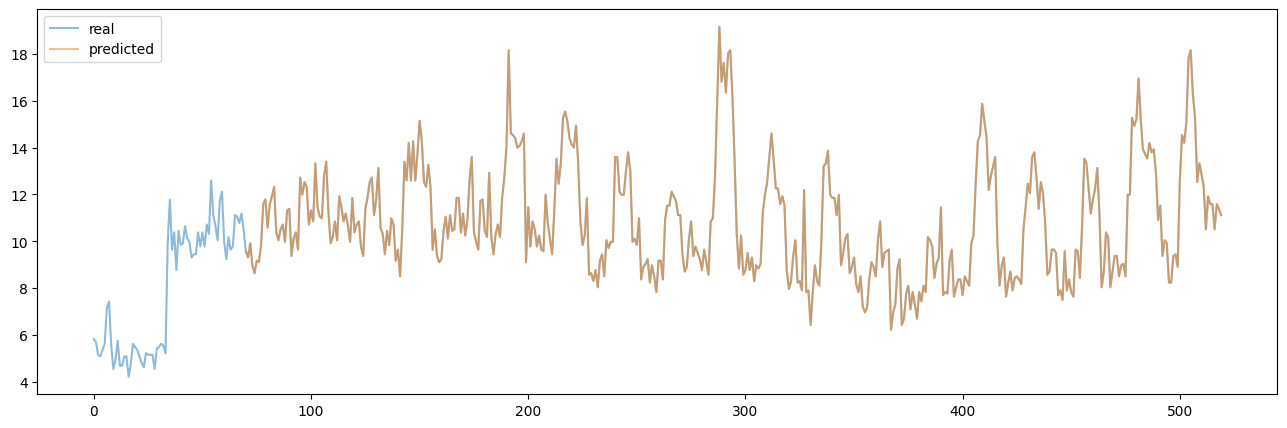
\includegraphics[width=\textwidth]{TwoTAlgo.png}
	\caption{Возвращение прогноза при идеальном прогнозе Sigma. $T=20$, $T'=10$}
	\label{fig:fig3}
\end{figure}

\subsection{Алгоритм при неидеальном прогнозе}

Проблема вышеописанного алгоритма заключается в том, что при неидеальном прогнозе, пересечения может не быть. Более того, если брать два ответа с минимальным расстоянием, мы можем взять не ту пару ответов.

Вместо двух значений  $T$ и $T'$ предлагается брать $K$ значений.

Тогда мы молучим $K$ наборов ответов:

\begin{gather*}
	[ans_{11}, ans_{12}],\\
	[ans_{21}, ans_{22}],\\
	\vdots \\
	[ans_{K1}, ans_{K2}]
\end{gather*}

Далее предлагается перебрать $2^K$ наборов ответов и выбрать тот набор, в котором диаметр минимален.

Асимптотическая сложность данного восстановления будет $O(2^K \times K \times N)$ + сложность используемого алгоритма поиска минимума.

\begin{figure}
	\centering
	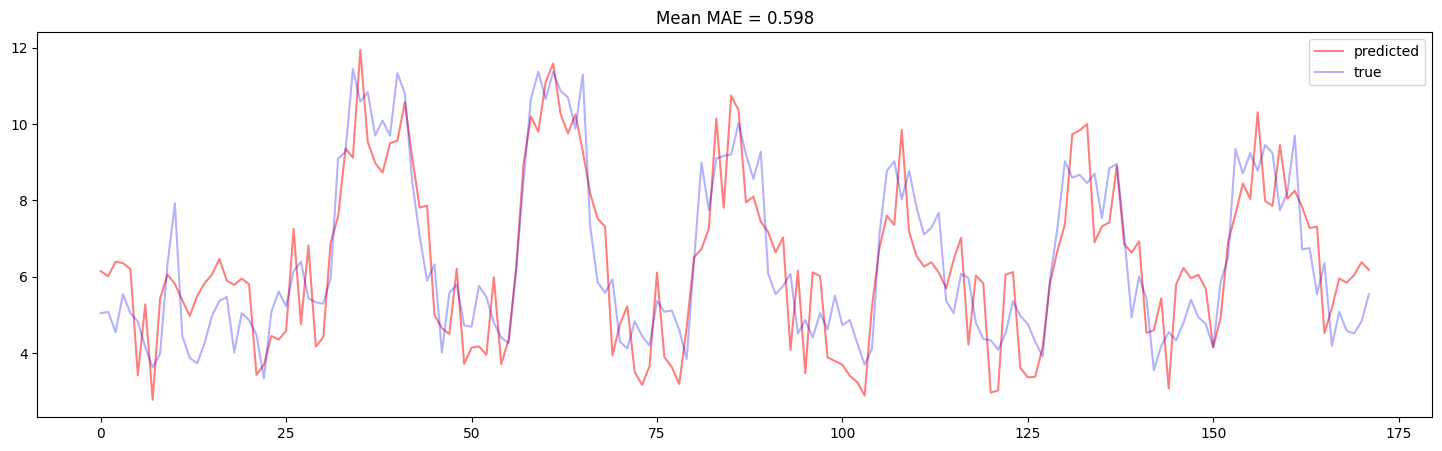
\includegraphics[width=\textwidth]{TbiLSTM.png}
	\caption{Возвращение прогноза при неидеальном прогнозе Sigma при помощи Bidirectional LSTM}
	\label{fig:fig4}
\end{figure}

\textbf{TODO Математическая логика}

\section{Computational Experiment}

Исследуются следующие алгоритмы прогнозирования:

\begin{itemize}
	\item LSTM \cite{LSTM}
	\item SARIMA \cite{ARIMAvsLSTM}
	\item LSTM на матрице расстояний
	\item Bidirectional LSTM на матрице расстояний
\end{itemize}

\subsection{LSTM}

LSTM, в отличии от обыкновенной RNN позволяет выделять как кратковременные, так и долговременные зависимости, что позволяет с довольно высокой точностью прогнозировать временные ряды.

В качестве теста используется зашумленный временной ряд длины T, состоящий из суммы синусов и косинусов разных амплитуд и сдвигов. Из этого временного ряда генерируется выборка следующим алгоритмом:\\
1. Выбирается размер окна $W$.\\
2. Ряд разбивается на $T-W-1$ окон размера $W+1$ со сдвигом 1. Эти окна будут семплами\\
3. В каждом из полученных окон первые $W$ будут аргументами на данном семпле, а последнее~--- результатом.

Ряд восстанавливается неплохо, однако минусом является то, что при усложнении данных сильно растёт сложность модели. Так же, LSTM не может работать с многомерными рядами.

\subsection{SARIMA}

ARIMA позволяет находить авторегрессионные зависимости. SARIMA (Seasonal ARIMA) учитывает так же сезонность данных. Это может быть полезным в случае с данными природного характера, как например, температура воздуха или выработка электричества.

Ряд прогнозируется довольно плохо, в случае если он имеет достаточно нетривиальную структуру. Так же, в данных может не быть явной сезонности, что ухудшает точность данного метода.

\subsection{LSTM на матрице попарных корреляций}

\subsection{Bidirectional LSTM на матрице попарных корреляций}



\begin{figure}
	\centering
	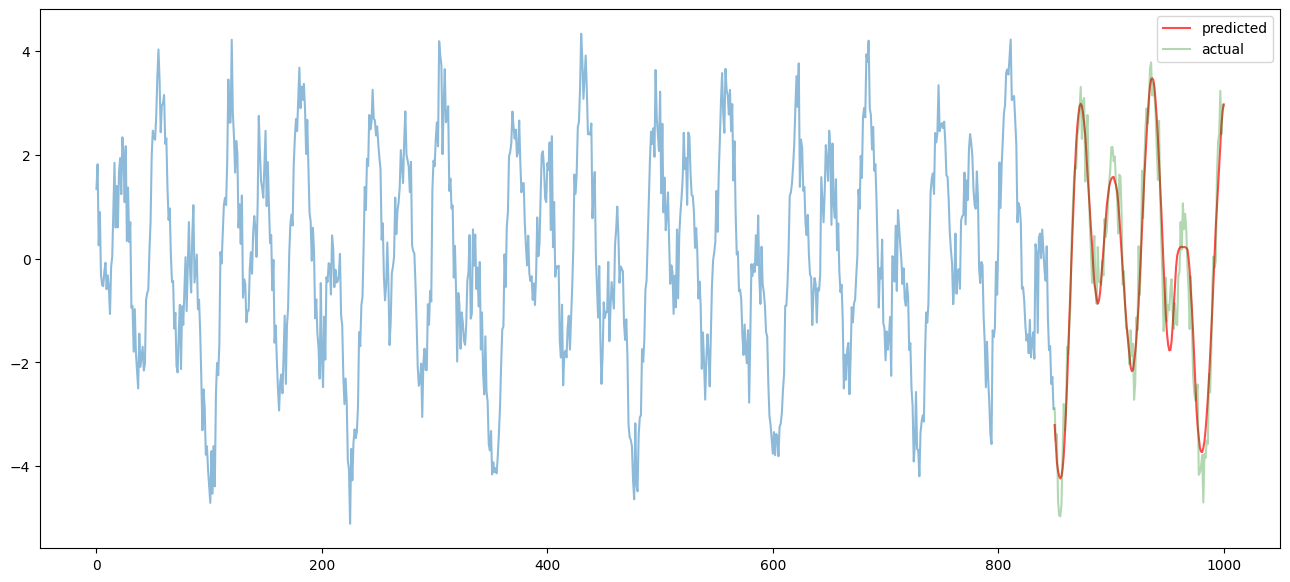
\includegraphics[width=\textwidth]{LSTM-prediction.png}
	\caption{Прогноз с использованием LSTM}
	\label{fig:fig1}
\end{figure}
\begin{figure}
	\centering
	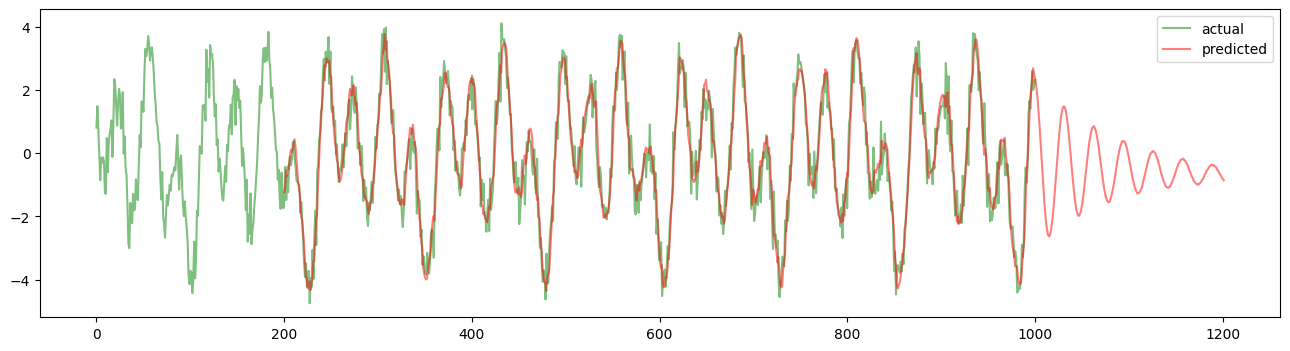
\includegraphics[width=\textwidth]{SARIMA-prediction.png}
	\caption{Прогноз с использованием SARIMA}
	\label{fig:fig2}
\end{figure}

\bibliography{references}
\bibliographystyle{plain}


\end{document}